\chapter{Results and Discussion}
This chapter gives provides the cross sections obtained from the analysis described in the last chapter, for $^\text{nat}$Ir(d,x) in section \ref{sec:ir_crossSections}, ... 

The observed products were....... 


In general, the products which were expected to be observed was observed, with a few exceptions which were mainly due to short counting time, and lack of strong independent gamma-lines. This was in particular evident for the iridium products, where only (d,n) and (d,p) reactions were observed. The Coulomb barrier constraint is taller for a heavier target-isotopes \ref{eq:Coulomb_barrier}, and for the compound nuclei of platinum, the alpha-barrier was approximately 27 MeV, and the proton barrier was approximately 13 MeV. In comparison, the alpha-barrier for the compound nuclei produced from the monitor foils was approximately 10 MeV and the proton barrier was approximately 7 MeV. Whenever a reaction is above an energetic threshold, the reaction does occur. But the since the total cross section of production of the compound nucleus is the sum of all possible reactions which is a more or less constant value, other reaction channels are fed, like the emission of protons and neutrons. The high barrier suggests that it is difficult to extract alpha-particles in the deuteron energy region up to 33 MeV, but as long as the reaction is above threshold, a chance of tunneling is present. This implies that extracting more than one proton would have a higher probability, which was not observed in this work. Conclusion is however that the cross section is so low that it was observed. \\


Then the reactions from monitor foils. 


For all reaction channels in each type of target, it was clear that the decay channels with emission of deuterons, tritons and $^3$He had very low cross sections, and was for most reactions not observed. Instead, the reaction channels of neutron and proton emission along with alpha-particles were more fed, with the proton and neutrons having the highest cross section, as described in the theory for compound nuclear reactions. Alpha-particles are preferred for emission because of the low binding energy along with the ..

For all the reactions, the energy level, half-life, decay-mode, Q-values, the gamma-ray energies and intensities are listed in tables \ref{tab:Products_Fe}, \ref{tab:Products_Ni}, \ref{tab:Products_Cu} and \ref{tab:Products_Ir} for iron-products, nickel-products, copper-products and iridium-products respectively. 

The uncertainty in cross section was calculated as the quadruple sum of each term in equation .... The main difference in each foil was the induced activity, since the other values are constant for each single reaction. 


\section{Cross section of $^\text{nat}$Ir(d,x)-reactions} \label{sec:ir_crossSections}

The production of $^{191,193}$Os ($t_{1/2}$=15.4 d (ground-state), 30.11 h, respectively) \cite{Vanin2007, ShamsuzzohaBasunia2017a} via alpha-emission or emission two protons was expected, due to the low energy threshold of the reactions $^{191}$Ir(d,2p)$^{191}$Os (Q=-1.8 MeV) or $^{193}$Ir(d,$\alpha$)$^{191}$Os (12.6 MeV) and $^{193}$Ir(d,2p)$^{193}$Os (Q=-2.6 MeV)\cite{PritychenkoB.SonzogniA.NNDC}. $^{191}$Os has one strong gamma-line (129.431 keV, 26.50\%) which is shared with $^{191}$Pt ($t_{1/2}$=2.802 d) (both nuclides decay to stable $^{191}$Ir)\cite{Vanin2007}. This radionuclide have been observed by Tárkányi et. al. (2019) \cite{Tarkanyi2019}, and the suggestion that this radionuclide was not observed in this work was because the iridium-foils were not counted sufficiency long for the $^{191}$Pt to decay completely. The cross sections provided by Tárkányi et. al. (2019) are however low, ranging from zero to 1.85 mb for deuterons up to 34.52 MeV. $^{193}$Os was not observed, and the main suggestion for this is that the gamma-lines of the nucleus are weakly fed, combined with that the reaction cross section is weak. In addition to expected osmium radionuclides, rhenium and tungsten was also expected to be produced in a sufficient amount for observation via the (d,x$\alpha$p) or (d,x$2\alpha$) reaction channels, but was not observed. In particular, multiple gamma-lines present in rhenium were observed, but since products of iridium with the same mass number fed into the same nucleus of osmium, it was not possible to make independent observations of either, even though the gamma-lines were more intense for rhenium than for iridium radionuclides. As a consequence of osmium not being observed suggests that the amount produced of the radionulides of rhenium and tungsten was not high enough either. \\

The independent cross sections were measured for $^{188,189, 191, 193m}$Pt and $^{188,194m2}$Ir, along with the cumulative cross sections for $^{188,189,190, 190m1+g, 192,194}$Ir, which are described below. The data is compared to data from Tárkányi et. al. (2016, 2019) \cite{Tarkanyi2006a, Tarkanyi2019} who have performed two similar experiments with deuteron energy in the ranges 1.7-38.0 MeV and 17.09-49.50 MeV  respectively. 

\subsection{$^\text{nat}$Ir(d,x)$^{188}$Pt (independent)}
$^{188}$Pt ($t_{1/2}$=10.2 d) decays by electron capture/$\beta^+$ to $^{188}$Ir. This nuclide was produced via $^{191}$Ir(d,5n) \cite{Kondev2018} (Q=-26.1 MeV). The first measured point was at beam energy 26.03 MeV, and as can be seen on figure \ref{fig:188Pt} and in table \ref{tab:Iridium_Cross_sections}, the measured points are low and in the threshold region. There is no previous experimental data in this region, however Tárkányi et. al. (2006) published measured cross sections at deuteron energies 13.1 and 16.5 MeV, which is nonphysical regarding that the energetic threshold for the reaction is much higher. The remaining data however agrees with an increase in the compound peak following threshold. The TENDL-2019, TALYS-1.9, ALICE-2017 and CoH-3.5.3 agrees in where the threshold for the reaction is, but disagrees in the slope of the curve. TENDL-2019 and CoH-3.5.3 is in best agreement with the previous data. TALYS-1.9 clearly underestimates the magnitude of the compound peak, and EMPIRE-3.2.3 overestimates the threshold and underestimates the slope. \\

The activity curve was obtained using the relatively intense gamma-lines listed in table \ref{tab:Products_Ir}, using a single-decay fit. The lines were not contaminated by background radiation or by other nuclei. The relative uncertainty in the end of beam activity was 13.6\%, 28.2\% and 26.6\% in foil 1,2 and 3 respectively, which contributes to a larger net-uncertainty in the final cross section. The large uncertainty caused by the low production of the radionuclide in the foils and therefor due poor statistical observations in the gamma-ray spectra, which were as high as 50\%. 

\begin{figure}
    \centering
    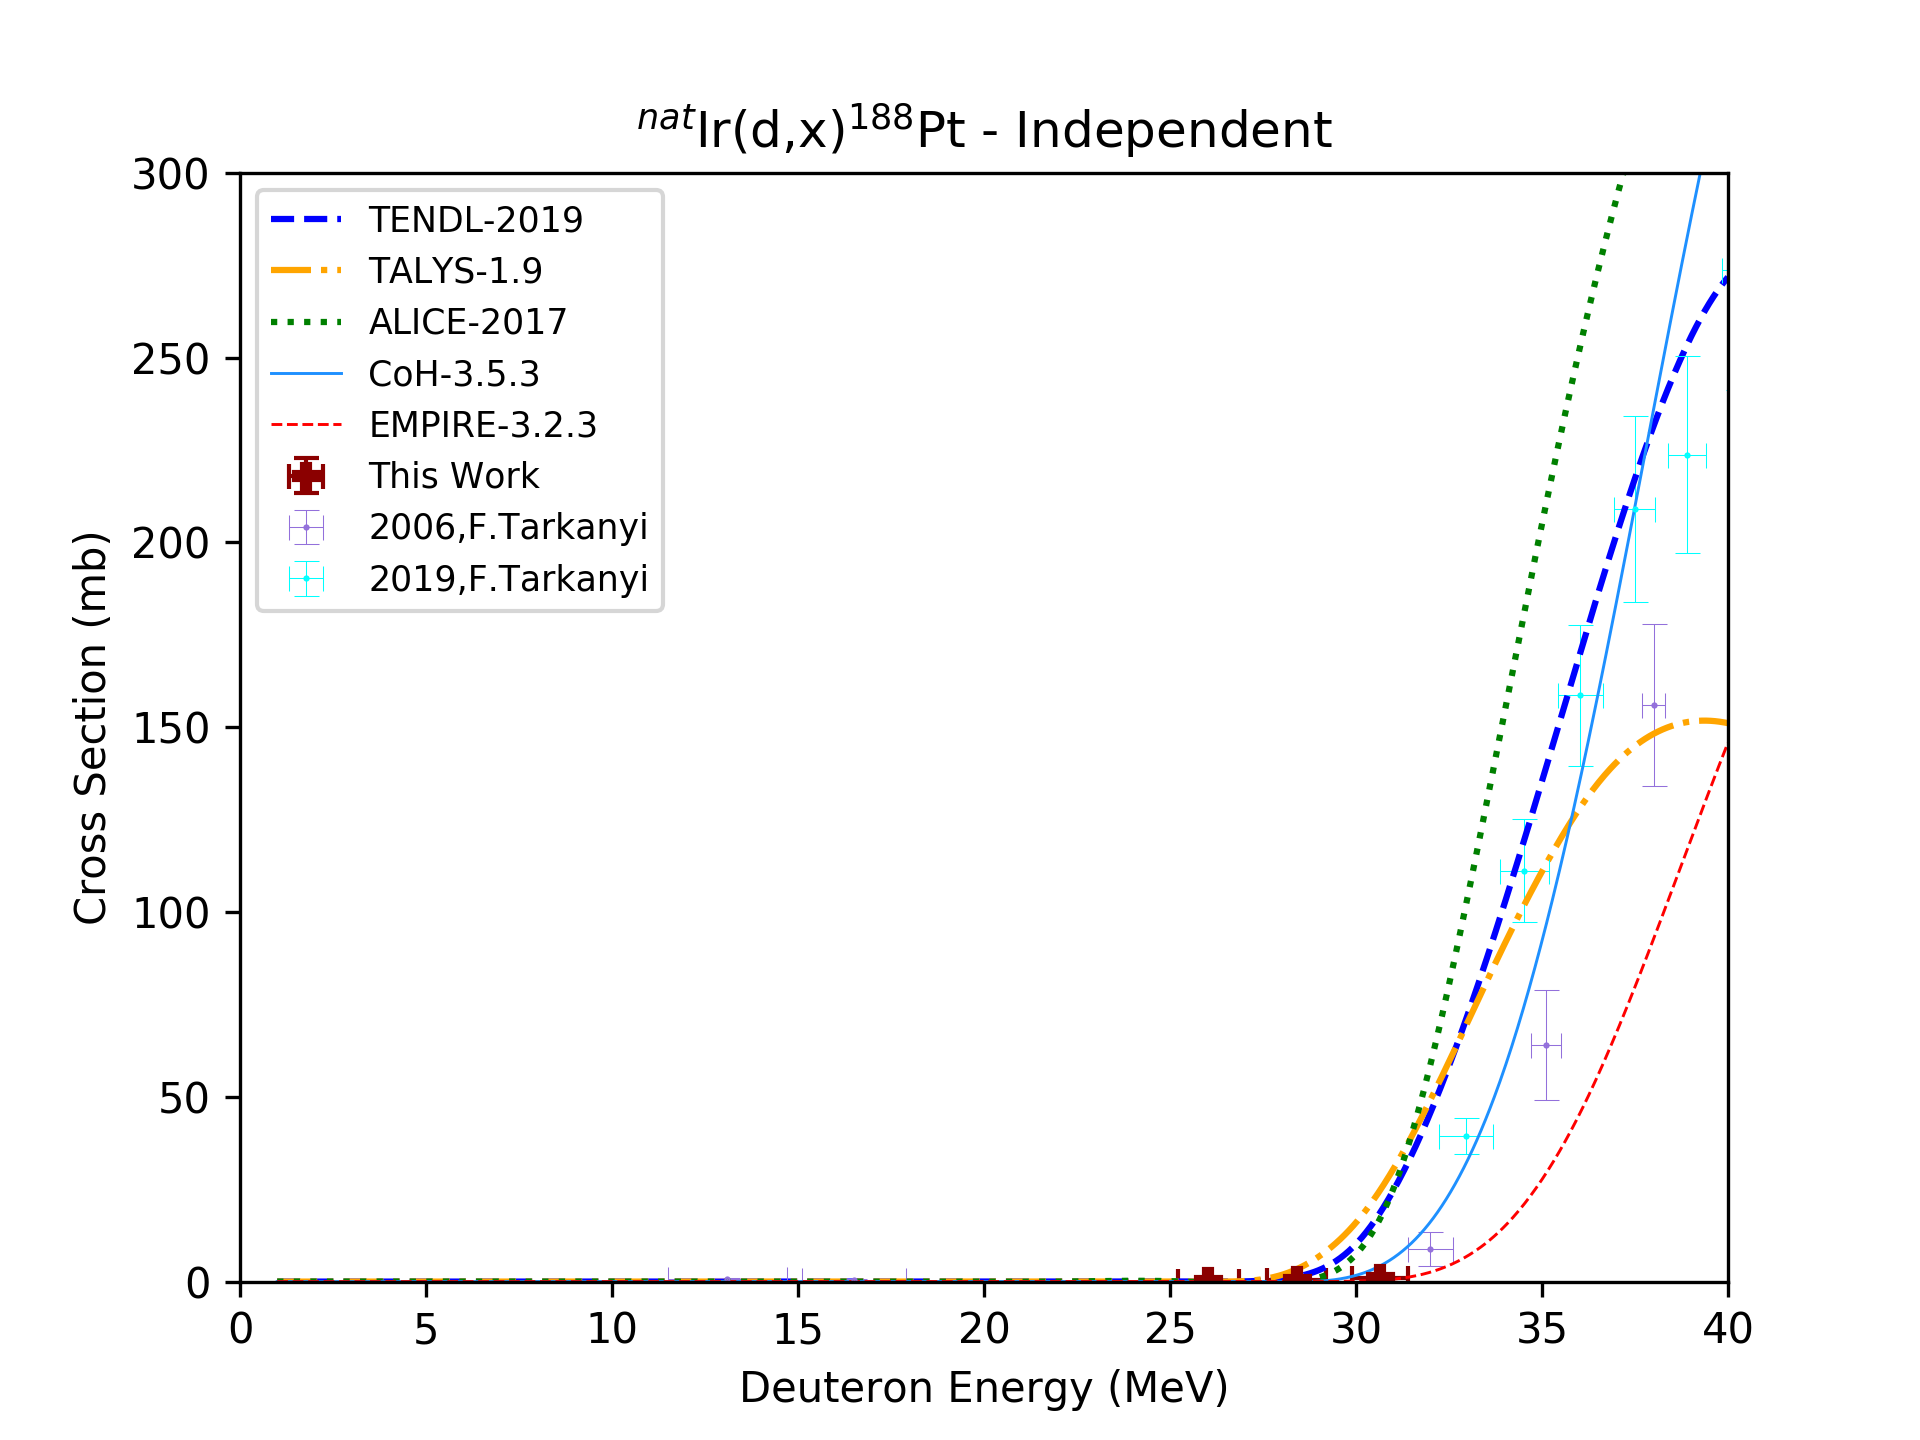
\includegraphics{Results/Ir_188Pt.png}
    \caption{The figure shows the measured cross sections as a function of the weighted average beam energy in iridium, along with experimental data from Tárkányi et. al. (2006, 2019) \cite{Tarkanyi2006a, Tarkanyi2019}, along with reaction modeling codes. }
    \label{fig:188Pt}
\end{figure}

\subsection{$^\text{nat}$Ir(d,x)$^{189}$Pt (independent)}
$^{189}$Pt ($t_{1/2}$=10.87 h) decays by electron capture/$\beta^+$ to $^{189}$Ir. This radionuclide can be produced via $^{191}$Ir(d,4n) \cite{Johnson2017} (Q=-19.3 MeV) with the deuteron beam energies in this experiment. The first measured cross section was at beam energy 19.03 MeV. Figure \ref{fig:189Pt} shows the measured cross section along with the experimental data and reaction models. The measured cross sections in this work agrees well with the experimental data up to beam energy 23.54 MeV, and after, the values are higher. The reaction models disagree on the exact location of the compound peak,where CoH-3.5.3 follows performs best magnitude-wise and EMPIRE-3.2.3 follows the shape best. The increase in cross section after the compound peak is the opening of the next reaction channel from $^{193}$Ir(d,6n) which had an energetic threshold larger than the deuteron beam used in this experiment. TALYS-1.9 underestimates both the peak location, width and magnitude, and performs poorest here. \\

The activity curve was obtained using the relatively intense gamma-lines (higher than 1\%) listed in table \ref{tab:Products_Ir}, which were not contaminated by background or by other nuclei. The activities as a function of time since EOB was fitted to a single-decay curve. The relative uncertainty in EOB activities were below 4\% for the four first foils, and increasing to 6.1\% in foil 5 and to 25.7\% in foil 6, where the cross section is low and the reaction is around threshold, and the statistical uncertainty in number of counts are is large.   

\begin{figure}
    \centering
    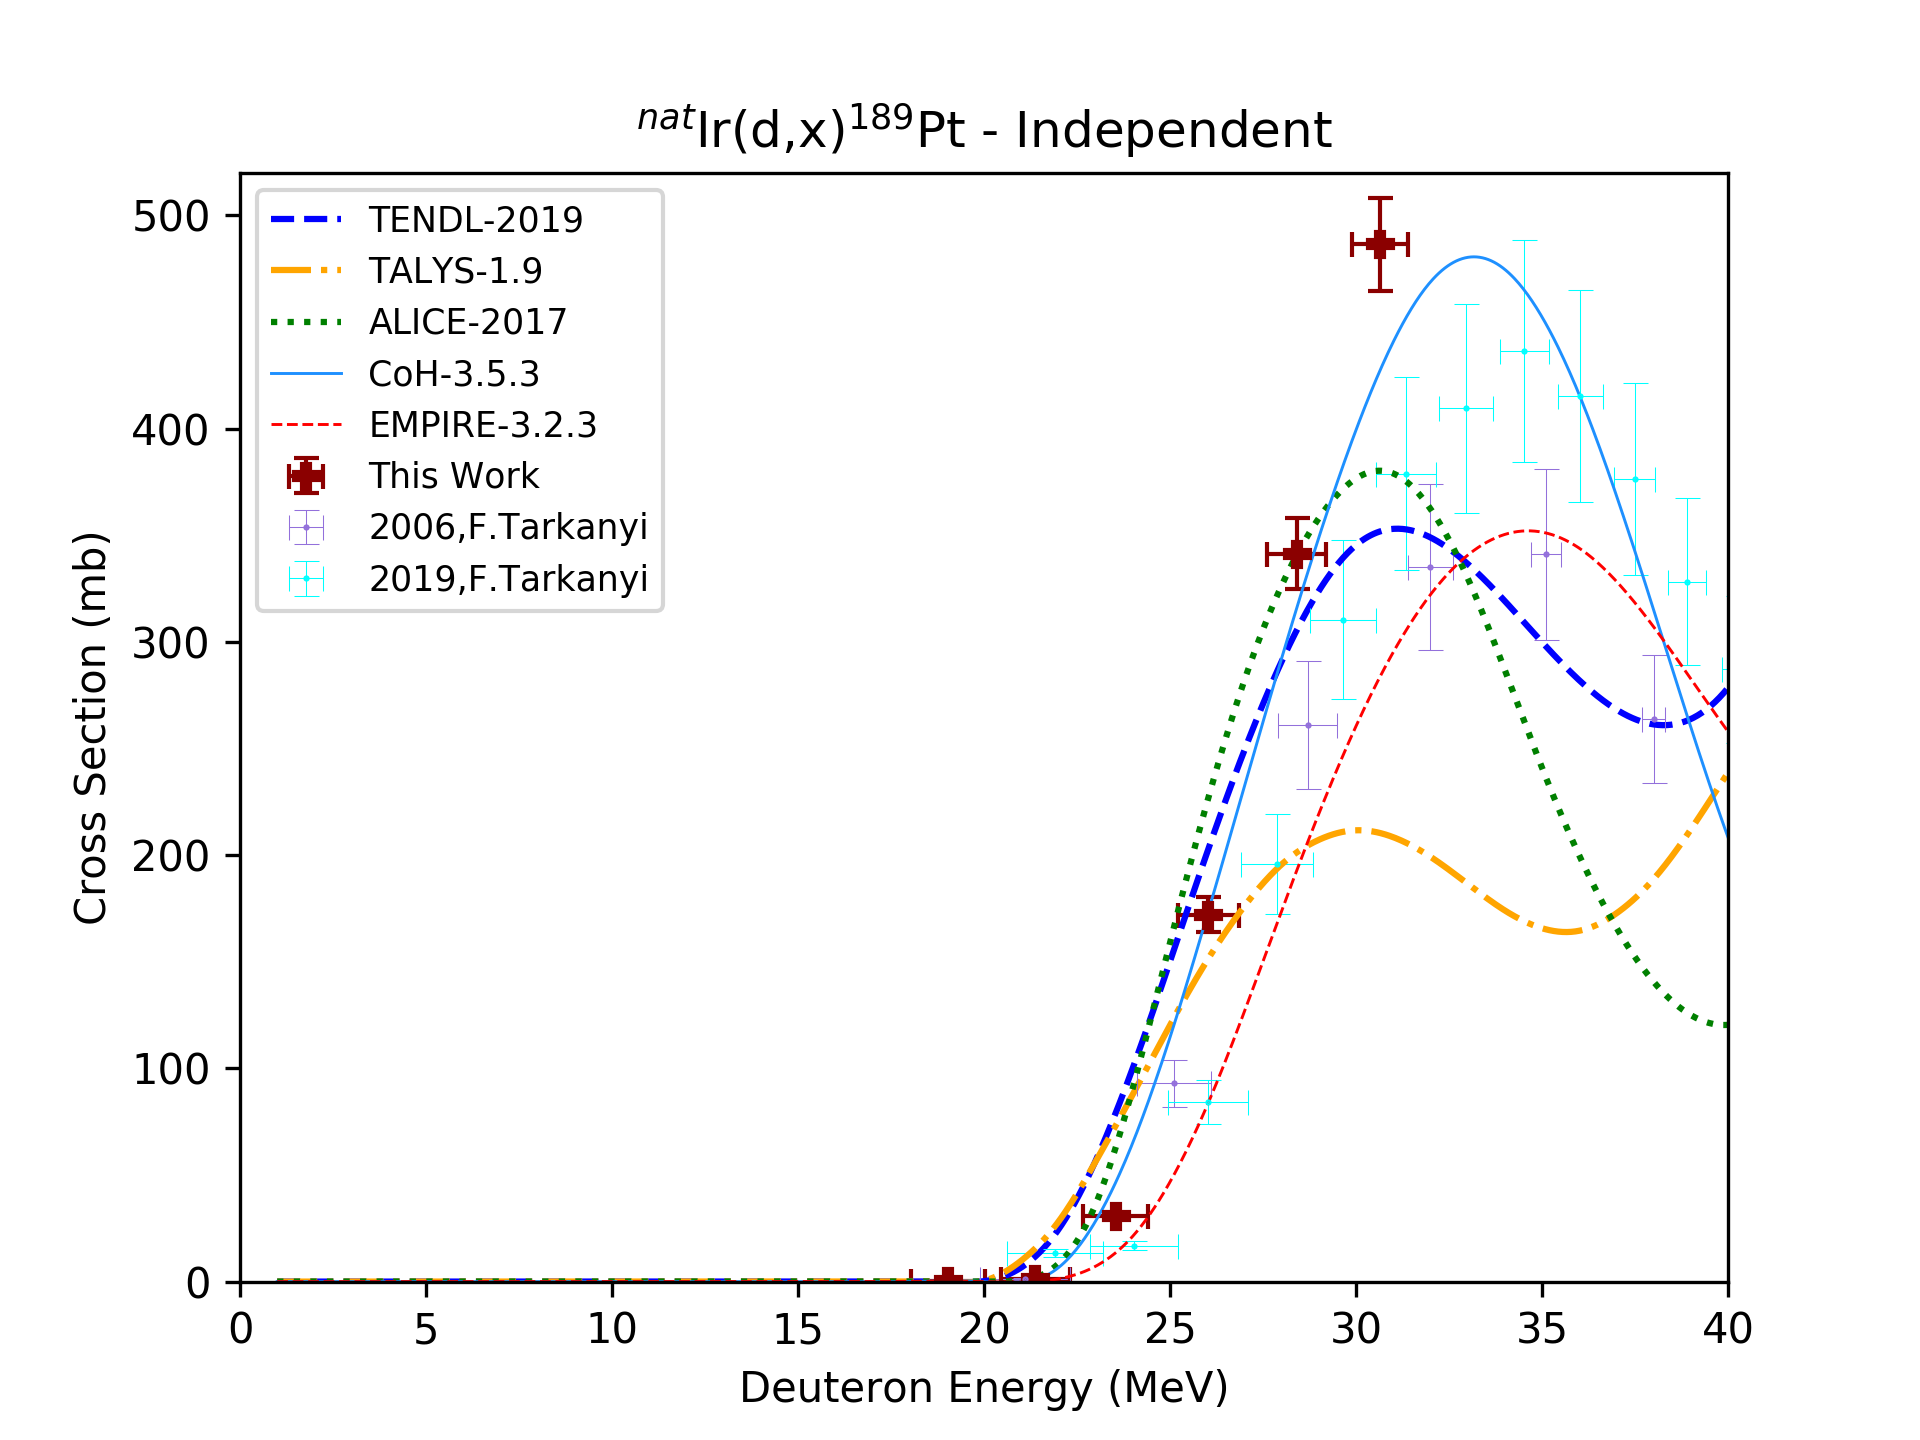
\includegraphics{Results/Ir_189Pt.png}
    \caption{---}
    \label{fig:189Pt}
\end{figure}




\begin{group}
\setlength{\tabcolsep}{2pt} % Default value: 6pt
\renewcommand{\arraystretch}{1.5} % Default value: 1
\begin{table}[]
    \scriptsize
    \centering
    \begin{tabular}{lllllllllll}
    \hline
     \makecell{E_d} & \makecell{30.03^{+0.67}_{-0.67}} & \makecell{28.40^{+0.80}_{-0.79}} & \makecell{26.03^{+0.82}_{-0.82}} & \makecell{23.54^{+0.88}_{-0.87}} & \makecell{21.38^{+0.94}_{-0.92}} & \makecell{19.03^{+1.00}_{-0.99}} & \makecell{16.43^{+1.11}_{-1.08}} & \makecell{13.51^{+1.28}_{-1.22}} & \makecell{10.09^{+1.55}_{-1.41}} & \makecell{5.63^{+2.21}_{-1.83}} \\
    \Xhline{2\arrayrulewidth}
     \makecell{$^{188}$Pt$_i$} & \makecell{0.94 (0.13)} & \makecell{0.30 (0.09)} & \makecell{0.17 (0.05)} & \makecell{-} & \makecell{-} & \makecell{-} & \makecell{-} & \makecell{-} & \makecell{-} & \makecell{-} \\
     \makecell{$^{189}$Pt$_i$} & \makecell{486.47 (21.86)} & \makecell{341.24 (16.64)} & \makecell{172.11 (8.03)} & \makecell{30.72 (1.48)} & \makecell{1.04 (0.07)} & \makecell{0.09 (0.02)} & \makecell{-} & \makecell{-} & \makecell{-} & \makecell{-} \\     
    \end{tabular}
    \caption{Caption}
    \label{tab:Iridium_Cross_sections}
\end{table}
\end{group}

\begin{comment}
\begingroup
\setlength{\tabcolsep}{10pt} % Default value: 6pt
\renewcommand{\arraystretch}{1.5} % Default value: 1
\begin{table}[]
\caption{....}
    \centering
    %\footnotesize
    \begin{tabular}{c  c c c c c c}
        \hline
        & \multicolumn{4}{c}{ \underline{Production cross section (mb) for ... }}\\
        %\hline
       \makecell{$E_d$ (MeV)}   & \makecell{$^{59}$Fe$_\text{cum}$} & \makecell{$^{60}$Co$_\text{cum}$} & \makecell{$^{61}$Co$_\text{cum}$} & \makecell{$^{65}$Ni$_\text{ind}$}  & \makecell{$^{61}$Cu$_\text{cum}$} & \makecell{$^{64}$Cu$_\text{ind}$} \\ 
       \makecell{30.03_{-0.67}^{+0.67}} & \makecell{0.21 \pm 0.03} & \makecell{9.49 \pm 0.52} & \makecell{1.62 \pm 0.09} & \makecell{3.42 \pm 1.76} & \makecell{4.54 \pm 0.87} & \makecell{170.76 \pm 7.76} \\
       \makecell{27.74_{-0.71}^{+0.72}} & \makecell{0.18 \pm 0.02} & \makecell{11.38 \pm 0.51} & \makecell{0.82 \pm 0.07} & \makecell{3.84 \pm 1.94} & \makecell{2.07 \pm 0.95} & \makecell{153.78 \pm 8.20} \\
       \makecell{25.32_{-0.76}^{+0.77}} & \makecell{0.17 \pm 0.02} & \makecell{12.02 \pm 0.51} & \makecell{0.29 \pm 0.05} & \makecell{2.89 \pm 1.48} & \makecell{1.18 \ pm 0.72} & \makecell{132.56 \pm 6.93} \\
       \makecell{22.77_{-0.81}^{+0.83}} & \makecell{0.12 \pm 0.01} & \makecell{11.36 \pm 0.43} & \makecell{-} & \makecell{1.92 \pm 1.14} & \makecell{-} & \makecell{121.54 \pm 7.12} \\
       \makecell{20.57_{-0.87}^{+0.89}} & \makecell{0.07 \pm 0.01} & \makecell{9.27 \pm 0.41} & \makecell{-} & \makecell{-} & \makecell{-} & \makecell{106.07 \pm 5.81} \\
       \makecell{18.14_{-0.94}^{+0.97}} & \makecell{0.03 \pm 0.01} & \makecell{5.65 \pm 0.26} & \makecell{-} & \makecell{1.46 \pm 0.95} & \makecell{-} & \makecell{95.92 \pm 7.14} \\
       \makecell{15.43_{-1.04}^{+1.08}} & \makecell{-} & \makecell{1.53 \pm 0.12} & \makecell{-} & \makecell{-} & \makecell{-} & \makecell{123.79 \pm 6.62} \\
       \makecell{12.34_{-1.20}^{+1.27}} & \makecell{-} & \makecell{-} & \makecell{-} & \makecell{-} & \makecell{-} & \makecell{156.65 \pm 8.20} \\
       \makecell{8.68_{-1.43}^{+1.62}} & \makecell{-} & \makecell{-} & \makecell{-} & \makecell{-} & \makecell{-} & \makecell{209.38 \pm 11.27} \\
       \makecell{3.94_{-2.22}^{+2.25}} & \makecell{-} & \makecell{-} & \makecell{-} & \makecell{-} & \makecell{-} & \makecell{73.54 \pm 5.70} \\
    \end{tabular}
    \label{tab:crossSections_Pt}
\end{table}
\endgroup
\end{comment}




